% Select Times-compatible T1 fonts before IEEEtran, including under Tectonic/XeTeX.
\RequirePackage[T1]{fontenc}
\documentclass[conference]{IEEEtran}
\usepackage{cite}
\usepackage{graphicx}
\usepackage{array}
\usepackage{amsmath,amssymb,amsfonts}
\usepackage{textcomp}
\usepackage{url}
\usepackage[hidelinks]{hyperref}
\usepackage{xcolor}
\emergencystretch=3em
\setcounter{dbltopnumber}{2}
\renewcommand{\dbltopfraction}{0.95}
\renewcommand{\dblfloatpagefraction}{0.85}
\renewcommand{\textfraction}{0.05}
\newcommand{\CADDAM}{CADD\allowbreak{}+\allowbreak{}AlphaMissense}
\newcommand{\GCNCADDAM}{GCN\allowbreak{}+\allowbreak{}CADD\allowbreak{}+\allowbreak{}AlphaMissense}

\title{Auditing PPI Graph Augmentation for Missense Variant Pathogenicity Prediction under Topology, Connectivity and Homology Constraints}

\author{}
\hypersetup{pdfauthor={}}

\begin{document}
\maketitle


\begin{abstract}
\bfseries\boldmath
We evaluate fixed two-hop protein-feature propagation (FPP) for missense variant pathogenicity prediction using 177,213 ClinVar variants, an external UniProt source and two networks. Only the downstream classifier is trained. Matched STRING controls show sensitivity to connectivity and protein--topology correspondence. On the original split, STRING fusion improves over raw-embedding fusion, whereas its added value over strong variant scores remains uncertain under homology-aware splitting. On 10,785 external variants, STRING increases the mean area under the receiver operating characteristic curve from 0.6932 to 0.7304; the ensemble gain is +0.0375 with a protein-bootstrap 95\% interval of [+0.0173, +0.0564]. A stricter nested subset supports the same direction. For BioGRID, external gains over raw embeddings and incremental gains over raw-embedding fusion remain uncertain. The findings support STRING transfer under the stated exclusions and show that graph-associated gains depend on the network, comparator and split. They concern transductive protein-context features and should not be generalized to trained graph neural networks.

\end{abstract}

\begin{IEEEkeywords}
\bfseries\boldmath
Missense variant pathogenicity, STRING networks, fixed feature propagation, protein language models, evaluation audit.
\end{IEEEkeywords}

\section{Introduction}

Missense variant pathogenicity prediction has been advanced by established methods such as CADD, REVEL, MVP, PrimateAI, EVE and AlphaMissense \cite{Kircher2014CADD,Ioannidis2016REVEL,Qi2021MVP,Sundaram2018PrimateAI,Frazer2021EVE,Cheng2023AlphaMissense}, as well as by protein language models such as ESM \cite{Lin2023ESM}. These approaches capture sequence, evolutionary and annotation-derived signals. Disease-associated proteins are also embedded in molecular interaction networks, and disease-associated mutations can perturb protein-protein and other macromolecular interactions \cite{Barabasi2011NetworkMedicine,Menche2015DiseaseModules,Sahni2015InteractionPerturbation,Chen2018InteractomePerturbation}. PPI graphs provide an additional source of context for missense variant prediction.

Earlier approaches incorporated protein-interaction and other molecular-network features into single-amino-acid variant prioritization, showing that network context can provide information complementary to sequence, structure and annotation features \cite{Yates2014SuSPect,Ozturk2022NetworkFeatures}. More recent graph-based variant predictors include graph attention models for missense effects, heterogeneous gene-variant graph approaches, multimodal variant graph methods and disease-specific graph models \cite{Zhang2022gMVP,Cheng2021VEGN,Yu2025GNNMAP,Ghadie2025DiseaseSpecificGNN}. For fixed propagation over a shared STRING association graph, interpreting such gains requires separating network effects from information already present in the protein features.

Protein-disjoint train, validation and test partitions can remain directly connected in the shared STRING graph. Related proteins may also cross partitions when homology is not explicitly controlled \cite{Littmann2022ProteinMLTips,Teufel2023GraphPart}. Strong variant-effect predictors such as CADD and AlphaMissense can further reduce the marginal contribution of graph propagation. A graph-associated improvement therefore needs raw-embedding and strong-score controls, with uncertainty assessed at the protein level.

We compare raw ESM, fixed propagation, external scores and fusion models on the reconstructed ClinVar-STRING dataset using matched comparisons, graph interventions and protein-clustered uncertainty. External-source evaluation and a BioGRID comparison test transfer and sensitivity to network choice. Topology and error-transition profiles are exploratory. The audit does not introduce a new predictor or cover trained message-passing architectures.

\section{Materials and Methods}

\subsection{Dataset and graph construction}

ClinVar variant annotations were obtained from the official NCBI ClinVar FTP tab-delimited variant-summary file \cite{Landrum2020ClinVar}. All experiments used a frozen set of processed ClinVar tables identified by checksums; source provenance is documented in Supplementary Methods 1. We reconstructed a filtered, non-conflicting missense dataset and mapped variants to STRING human protein identifiers. We retained GRCh38 germline missense SNVs with criteria-supported review status, combined pathogenic and likely pathogenic records into the positive class, combined benign and likely benign records into the negative class, removed uncertain or conflicting records, and collapsed duplicate VariationIDs. The final ClinVar-STRING dataset contained 177,213 missense variants mapped to 14,123 labelled STRING proteins. The propagation graph contained 19,622 STRING protein nodes and 13,715,404 directed edge-index entries from the STRING v12 protein-association network \cite{Szklarczyk2023STRING}. STRING includes association evidence beyond direct physical interactions.

\subsection{Protein representations and fixed propagation}

Raw protein features were generated using the ESM-2 650M checkpoint, with 1,280-dimensional protein-level vectors obtained by residue averaging \cite{Lin2023ESM}. Fixed protein-feature propagation (FPP) was computed by two-hop GCN-style propagation over the normalized STRING graph \cite{Kipf2017GCN}. FPP has no learned graph-convolution parameters; the downstream MLP alone was trained. Fixed propagation isolates topology-induced smoothing from capacity gains due to trainable graph layers. Let $X$ denote the raw ESM protein-representation matrix. The matched implementation adds self-loops before symmetrizing the retained edge list and sums duplicate contributions when coalescing. Thus $\tilde{A}=(E+I)+(E+I)^{\mathrm{T}}$, where $E$ is the edge-index count matrix; STRING combined scores are not propagation weights. Let $\tilde{D}$ denote its weighted degree matrix. We computed the symmetrically normalized adjacency matrix as
\begin{equation}
\hat{A}=\tilde{D}^{-\frac{1}{2}}\tilde{A}\tilde{D}^{-\frac{1}{2}},
\end{equation}
\begin{equation}
H=\frac{1}{3}\left(X+\hat{A}X+\hat{A}^{2}X\right).
\end{equation}
The fixed two-hop FPP representation $H$ averages the original ESM features, one-hop and two-hop STRING-smoothed features. Downstream classification used the representation of each variant's mapped STRING protein. Propagation was transductive: it used only graph structure and ESM features from train, validation and test nodes, excluding held-out labels. Representation-only models were evaluated once per protein and assigned the same score to all its variants; they cannot resolve residue-specific effects within that protein. Ensemble probabilities were averaged in float64 before metric calculation.

\subsection{Splits, classifiers and external predictors}

The original split assigned train, validation and test variants by STRING protein ID, with no shared proteins across partitions. The split contained 141,864 training variants, 17,129 validation variants and 18,220 test variants. The homology-aware split used MMseqs protein clusters with minimum sequence identity 0.40, coverage 0.50 and coverage mode 0 \cite{Steinegger2017MMseqs2}. Each cluster was assigned wholly to one partition by greedy balancing of variant-row counts, without label-prevalence stratification, preserving the same row counts. We use this split as a stress test. Its test positive rate was 10.56\%, compared with 31.95\% in the original split, which limits direct cross-split AUPRC comparison.

All current comparisons used downstream MLPs with 512/128 hidden units, dropout 0.3 and validation-AUC checkpoint selection. Training used class-weighted binary cross-entropy and Adam with learning rate $10^{-3}$, weight decay $10^{-5}$ and batch size 1,024 \cite{Kingma2015Adam}. The positive-class weight was the training negative-to-positive count ratio. Classifier seeds 42--44, a maximum of 50 epochs and patience five were shared across arms; permutation controls crossed three graph permutations with the same classifier seeds. CADD v1.7 and AlphaMissense scores were matched to variant records \cite{Schubach2024CADDv17,Cheng2023AlphaMissense}. Missing values were imputed using training-set medians, with an AlphaMissense missingness indicator; inputs were not standardized. Models used the same hidden-layer architecture and preprocessing, although score-only models had fewer input-layer parameters. Training hyperparameters, score coverage and historical protocols are detailed in Supplementary Methods 3 and 5 and Tables 1 and 8.

\subsection{External-source and second-network validation}

We evaluated frozen classifiers trained on the original split using raw ESM, STRING FPP or BioGRID FPP. External evaluation used HUMSAVAR 2026\_03 from UniProtKB/\allowbreak{}Swiss-Prot, with no external fitting or tuning \cite{UniProt2025}. Pathogenic/likely pathogenic records were positive and benign/likely benign records negative; uncertain-significance records were excluded. Canonical sequences had to match a unique frozen graph node exactly, with the reference residue verified. We excluded original variants using the union of accession-, node- and gene-plus-substitution keys and dbSNP identifiers. The primary set excluded original training/validation proteins and identical full-length sequences: 10,785 variants from 2,498 proteins. A nested sensitivity set also excluded original test proteins and identical sequences: 6,934 variants from 1,713 proteins. All evaluated proteins remained nodes of the frozen transductive graph.

BioGRID 5.0.262 human physical-category records \cite{Stark2006BioGRID} were filtered to remove RNA-related methods and ambiguous mappings, then mapped to the same 19,622 nodes. The graph contained 931,458 unique undirected edges and 1,402 isolates; all test rows were retained. Nine additional classifiers covered BioGRID representation-only prediction and original/homology fusion, using the same operator, seeds and training budget. Of its edges, 56.54\% also occurred in STRING. Paired protein-bootstrap intervals used 2,000 resamples of three-seed mean probabilities, conditional on fitted models and without multiplicity adjustment. Full filtering, run verification and AUPRC results are in Supplementary Methods 6 and Tables 14--17.

\subsection{Audit analyses}

Uncertainty was assessed using variant-level bootstrap and protein-clustered bootstrap \cite{Efron1993Bootstrap}. Connectivity tests removed direct train-test STRING edges and regenerated FPP embeddings. Reference partial-ablation curves removed 0\%, 25\%, 50\%, 75\% and 100\% of direct train-test protein pairs using random removal, higher-STRING-score-first removal and lower-STRING-score-first removal. Topology permutation preserved the unlabeled graph structure and randomized the correspondence between protein identity and graph position, testing whether generic graph smoothing explained the gain. Fusion controls concatenated \CADDAM{} features with raw ESM, edge-ablated FPP and topology-permuted FPP representations, testing representation complementarity and sensitivity to protein-topology correspondence. Edge removal also changes normalization and retains indirect cross-partition paths; it does not isolate a causal contribution of direct connectivity.

All matched graph controls used the same self-loop convention and symmetric normalization operator as full FPP. The full-FPP representation was checked against the retained output. Implementation verification and the separate reference protocols are documented in Supplementary Methods 5.

Exploratory reference analyses stratified predictions by degree, k-core, betweenness, clustering and training-derived neighbour-risk features, and examined corrected and degraded predictions. Feature profiles are reported descriptively because the original variant-level tests did not account for repeated variants within proteins; multiplicity correction \cite{Benjamini1995FDR} does not resolve this dependence. AUPRC was computed as non-interpolated average precision and interpreted within each split because it depends on class prevalence \cite{Saito2015PrecisionRecall}.

\begin{table}[t]
\caption{Matched classifier fits and external evaluation. Repeats count fitted classifiers.}
\label{tab:run_sources}
\centering
\footnotesize
\setlength{\tabcolsep}{3pt}
\renewcommand{\arraystretch}{1.10}
\begin{tabular}{>{\raggedright\arraybackslash}p{0.37\columnwidth}>{\raggedright\arraybackslash}p{0.20\columnwidth}>{\raggedright\arraybackslash}p{0.35\columnwidth}}
\hline
Experiment & Repeats & Reported summary \\
\hline
Original-split representations & 3/arm$^*$ & Mean and sample SD \\
Original-split fusion & 3/arm$^*$ & Mean and sample SD \\
Homology-aware fusion & 3/arm & Mean and sample SD \\
BioGRID: three settings & 3/setting & Representation and both fusion splits \\
External-source evaluation & 3 models/arm & Frozen predictions; no fitting \\
\hline
\end{tabular}
\par\smallskip
\raggedright $^*$Permutation arms use 3 graphs $\times$ 3 seeds (9 fits). The 48 matched audit and 9 BioGRID fits share seeds 42--44 and a maximum of 50 epochs. Paired intervals use 2,000 bootstrap resamples of fitted ensemble predictions, not additional fits. Historical settings and reference estimates for Figs. 1E and 2D are in Supplementary Tables 2 and 8; full matched settings are in Methods 5--6 and Table 11.
\end{table}

\section{Results}

\subsection{Full-graph FPP gains and connectivity sensitivity}

With the matched protocol (Table~\ref{tab:run_sources}) and classifier seeds 42--44, raw ESM reached test AUC 0.7835 $\pm$ 0.0063 and AUPRC 0.6117 $\pm$ 0.0066; full FPP reached AUC 0.7950 $\pm$ 0.0016 and AUPRC 0.6485 $\pm$ 0.0117 (Fig. 1B). On ensemble-averaged predictions, the FPP-minus-ESM AUC difference was +0.0107, with protein-clustered 95\% CI [-0.0218, +0.0426]; the AUPRC difference was +0.0412, CI [-0.0106, +0.0767] (Fig. 1C). Variant resampling ignores within-protein dependence and gives a different uncertainty estimate. These intervals condition on the three fitted classifiers, rather than incorporating retraining variability.

Removing 1,242,422 direct train-test edge-index entries (9.06\%; 621,211 unique undirected pairs) and recomputing the same normalized operator gave edge-ablated FPP AUC 0.7702 $\pm$ 0.0077 and AUPRC 0.6077 $\pm$ 0.0140 (Fig. 1D). Repeating with three topology permutations by the same three classifier seeds gave pooled AUC 0.7803 $\pm$ 0.0092 and AUPRC 0.6103 $\pm$ 0.0084 (Fig. 1F). Per-graph and paired-seed results are retained separately in Supplementary Table 11. These comparisons share the propagation operator, classifier seeds and training budget. Edge removal also changes node degrees, while indirect cross-partition paths remain.

The historical partial-ablation curve (Fig. 1E) uses unmatched classifier settings, a different control operator and reused endpoints. It is descriptive and does not extend the matched comparison in Fig. 1D.

\begin{figure*}[!t]
\centering
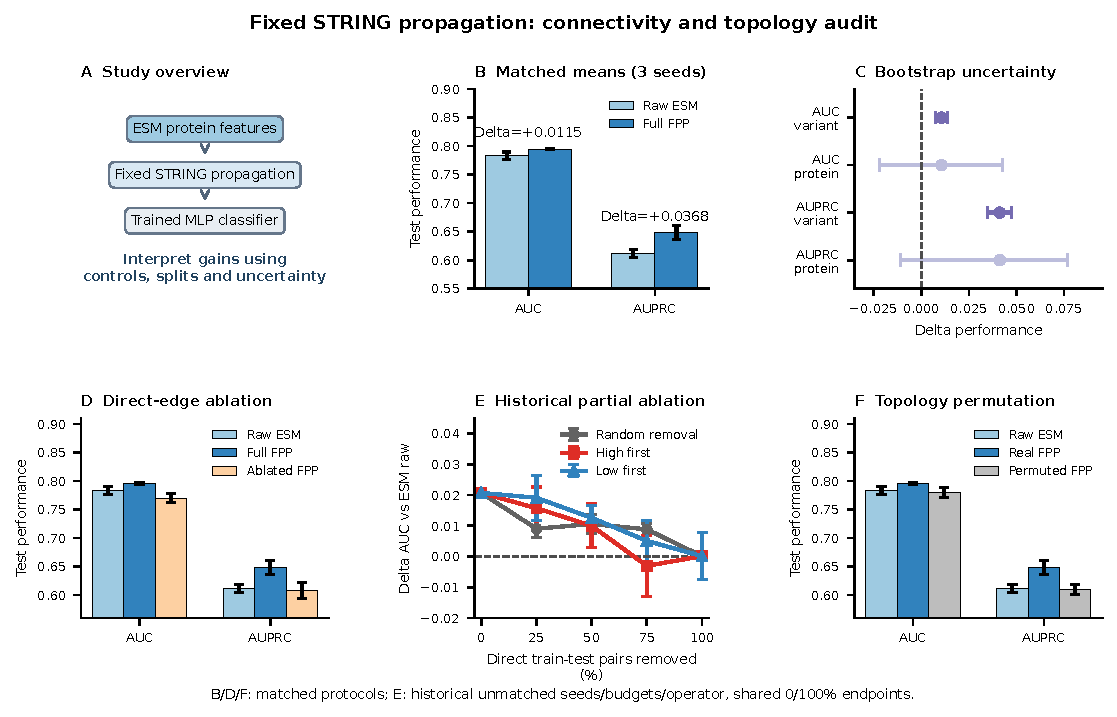
\includegraphics[width=0.98\textwidth]{figure_drafts/Figure1_fixed_propagation_audit.pdf}
\caption{Fixed STRING propagation audit. A, Study overview. B, Raw ESM and full FPP: mean and sample SD across three classifier seeds per arm. C, Paired bootstrap of three-seed mean probabilities, comparing variant and protein resampling; 2,000 replicates each. D, Direct-edge ablation with the common propagation operator and classifier protocol, mean and sample SD across three seeds. E, Historical partial-ablation curve with unmatched classifier settings, a different control operator and reused endpoints; this descriptive curve is not a matched continuation of D. F, Three topology permutations crossed with the same three classifier seeds; pooled mean and sample SD describe both sources of dispersion. The matched fits in B--D and F allow at most 50 epochs with validation-based early stopping; historical protocols are listed in Supplementary Table 8. Ensemble differences in C need not equal differences between mean run metrics in B.}
\label{fig:connectivity}
\end{figure*}

\subsection{Architecture-matched fusion and homology-aware stress test}

On the original split, mean AUC was 0.9572 for \CADDAM{}, 0.9682 with raw embeddings and 0.9716 with FPP (Fig. 2B). The ensemble FPP-minus-raw fusion margin had a protein-clustered 95\% interval of [+0.0008, +0.0062]. The edge-ablated margin remained uncertain, whereas the permutation margin was small and positive conditional on the sampled graphs (Fig. 2C; Supplementary Table 12). Intervals are exploratory, unadjusted for multiple comparisons and conditional on fitted models.

Figure 2D retains single-fit homology-aware representation estimates as reference context. The current homology-aware fusion comparison gave mean AUC 0.9755 for \CADDAM{}, 0.9727 with raw embeddings and 0.9752 with FPP, using three matched seeds per arm (Fig. 2E). The ensemble FPP-minus-score AUC difference was +0.0001, with protein-clustered 95\% CI [-0.0019, +0.0020]; the AUPRC interval also spanned zero (Supplementary Table 12). The incremental effect of STRING FPP over the score baseline remains uncertain under homology-aware splitting. Mean run metrics and metrics of averaged probabilities can give different close rankings.

\begin{figure*}[!t]
\centering
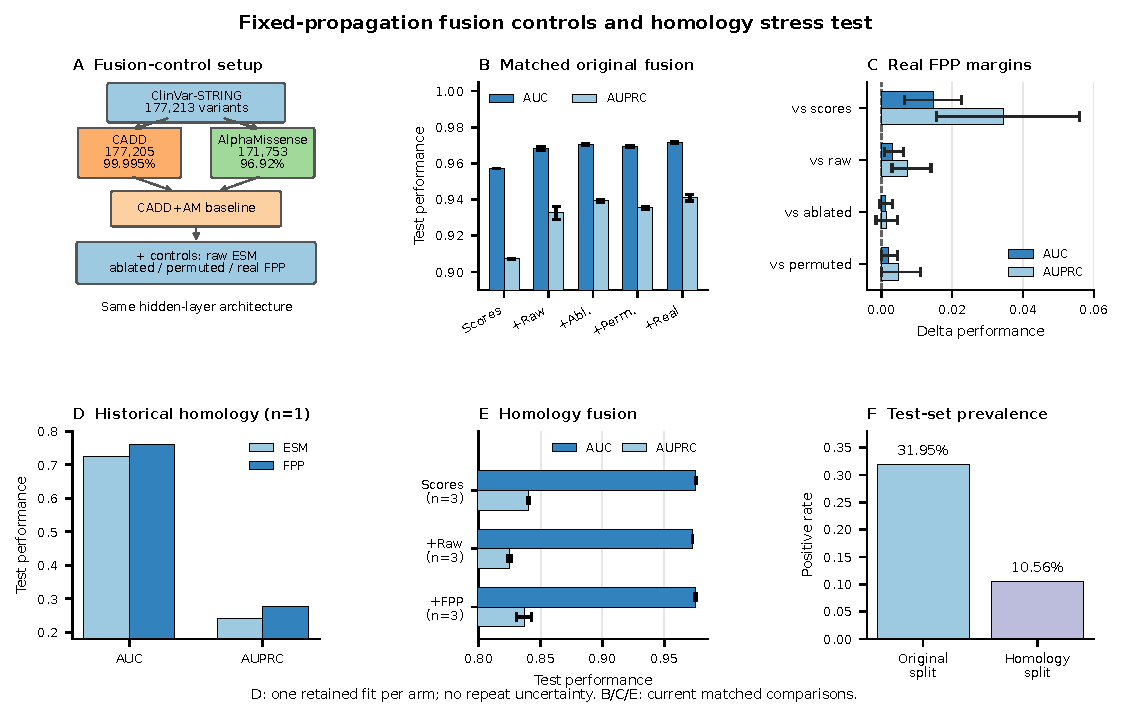
\includegraphics[width=0.98\textwidth]{figure_drafts/Figure2_fusion_homology.pdf}
\caption{Fusion controls and homology-aware evaluation. A, External-score coverage and fusion controls using the same hidden-layer architecture and training protocol. B, Original-split fusion, mean and sample SD across three classifier seeds per arm; the permutation control uses three graphs crossed with three seeds. C, Real-FPP minus control performance from mean probabilities, with paired protein-clustered 95\% bootstrap intervals (2,000 replicates). Intervals condition on fitted models and sampled graph permutations; they omit retraining and new-permutation uncertainty. D, Historical homology-aware representation estimates, one retained fit per arm without repeat uncertainty. E, Current homology-aware fusion under the same three seeds and training protocol, with sample SD. F, Test prevalence by split. Scores denotes CADD+AlphaMissense; Raw, Abl., Perm. and Real denote added representations.}
\label{fig:fusion_homology}
\end{figure*}

\subsection{External-source transfer and network dependence}

On the primary HUMSAVAR set, mean AUC across three seeds was 0.6932 for raw ESM, 0.7304 for STRING FPP and 0.7025 for BioGRID FPP. STRING-minus-raw ensemble differences were +0.0375 AUC (95\% CI [+0.0173, +0.0564]) and +0.0463 AUPRC ([+0.0151, +0.0745]). The stricter nested subset supported the same direction: +0.0352 AUC ([+0.0034, +0.0667]) and +0.0550 AUPRC ([+0.0111, +0.0962]). BioGRID-minus-raw intervals crossed zero on both sets (Fig.~\ref{fig:external}A; Supplementary Tables 16--17).

On the original ClinVar split, BioGRID representation-only mean AUC was 0.7592, compared with 0.7835 for raw ESM and 0.7950 for STRING. BioGRID fusion improved over scores alone (ensemble $\Delta$AUC +0.0124, CI [+0.0034, +0.0210]), but its incremental margin over raw-embedding fusion remained uncertain (+0.0009, [-0.0011, +0.0036]). BioGRID fusion was below STRING fusion in both original and homology splits under the fitted-ensemble intervals (Fig.~\ref{fig:external}B). In the homology split, its AUC interval against scores alone ended just below zero, while the AUPRC interval crossed zero. These comparisons show that the incremental value of propagation varies with the network and comparator.

\begin{figure*}[!t]
\centering
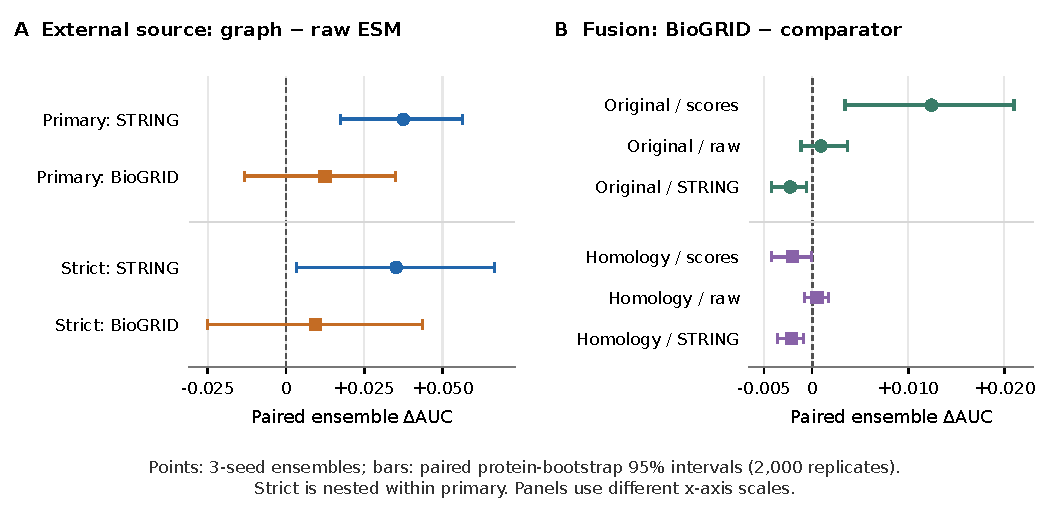
\includegraphics[width=0.98\textwidth]{figure_drafts/Figure3_external_validation.pdf}
\caption{External-source validation and alternative-network sensitivity. A, STRING- or BioGRID-FPP minus raw-ESM AUC on the primary HUMSAVAR set (10,785 variants; 2,498 proteins) and its stricter nested subset (6,934; 1,713). B, BioGRID fusion minus scores alone, raw-ESM fusion or STRING fusion, within each original or homology split. Points are differences in AUC of three-seed mean probabilities; bars are paired protein-clustered 95\% bootstrap intervals (2,000 resamples), conditional on fitted models. The dashed line marks zero. Axes use different scales. Strict is a sensitivity subset, not an independent replication. Intervals are exploratory and not adjusted for multiple comparisons.}
\label{fig:external}
\end{figure*}

\subsection{Exploratory topology and prediction changes}

Exploratory reference predictions showed non-monotonic gains across topology strata (Supplementary Fig. S2 and Table 5). All 53 joint cells and highlighted profiles were inspected on the same test set. Corrected and degraded predictions varied with the decision threshold and had different topology profiles (Supplementary Fig. S1 and Tables 6 and 10). These descriptive patterns motivate further evaluation; their interpretation remains limited by post-hoc selection and repeated variants within proteins.

\section{Discussion}

On the original split, fixed STRING propagation improved mean performance over raw ESM, but the protein-clustered intervals remained compatible with no gain (Fig.~\ref{fig:connectivity}C). Variants mapped to one protein share its representation, making protein-level resampling central to this interpretation. Edge removal and topology permutation probe different aspects of network context. Because edge removal also alters normalization and retains indirect paths, these interventions do not identify a causal effect of direct connectivity alone.

The homology-aware fusion comparison used three matched seeds per arm, and the STRING-versus-score intervals remained compatible with both benefit and harm. Redundant high-dimensional inputs, additional input weights, lack of feature scaling and altered protein composition could contribute to the uncertain fusion effect; these explanations were not experimentally separated. The frozen partition and differing prevalence limit broader cross-split conclusions.

External HUMSAVAR evaluation supports transfer of STRING protein-context features under explicit variant and protein exclusions. The BioGRID results leave both its external gain over raw embeddings and its incremental fusion gain over raw-embedding fusion unresolved. However, STRING incorporates evidence from multiple sources and overlaps BioGRID; their density, coverage, release and evidence composition differ. This comparison cannot isolate a causal effect of network identity or show that physical interactions are unhelpful.

HUMSAVAR and ClinVar may share underlying literature or annotations, so an external curated source is not an independent patient cohort or prospective validation. The strict set is nested, not a second replication; full homology separation and external-predictor development overlap were not excluded. Protein-only outputs cannot distinguish substitutions within a protein, and HUMSAVAR substitutions need not all be genomic SNVs. External clinical-score fusion was not evaluated. Fixed propagation does not establish what learned graph models could achieve. Selected topology profiles require independent confirmation; clinical use would additionally require calibration and decision-rule validation.

\noindent\textbf{Practical recommendations.}
Compare graph features with both raw protein embeddings and strong score baselines. Use the same training protocol across controls and report whether held-out proteins are visible in the graph. Quantify uncertainty at the protein level and check gains within the intended split. Treat selected subgroups as hypotheses, and evaluate calibration before using prediction changes to guide decisions.

\section{Conclusion}
Fixed STRING propagation improved external-source prediction under the specified exclusions and provided a small gain over raw-embedding fusion on the original split. Its added value over CADD+AlphaMissense remained uncertain under homology-aware splitting. For BioGRID, external gains and incremental fusion gains over raw-embedding controls remained inconclusive. Graph-derived gains should therefore be assessed for each comparator, split and network, with uncertainty quantified at the protein level. The findings concern fixed, non-trainable propagation in a transductive graph and should not be generalized to trained graph neural networks.

\section*{Data and Code Availability}

Supplementary Information and the reproducibility archive are publicly available; the identifying repository URL is withheld in this anonymous copy. The archive includes all 177,213 sample identities and split assignments, external membership flags, per-seed predictions, environment specifications, executed protocols, compact results and input checksums. Large provider resources, feature tensors and model checkpoints are retained separately. Data sources are ClinVar, STRING, CADD, AlphaMissense, UniProt and BioGRID.

\section*{Acknowledgment}

OpenAI ChatGPT, OpenAI Codex and Anthropic Claude assisted with literature organization, code development for the methods and analyses in Sections II--III and the Supplementary Methods, and language editing throughout the manuscript. AI-assisted scripts were used for environment restoration, data checks, model fitting and statistical analysis. The authors take responsibility for reviewing the code and outputs and for the study design, results, interpretation, references and final manuscript.

% Balance the final reference page using the IEEEtran class hook.
\IEEEtriggeratref{27}
\begin{thebibliography}{99}
\bibitem{Kircher2014CADD} M. Kircher et al., ``A general framework for estimating the relative pathogenicity of human genetic variants,'' \emph{Nature Genetics}, vol. 46, pp. 310--315, 2014, doi: 10.1038/ng.2892.
\bibitem{Ioannidis2016REVEL} N. M. Ioannidis et al., ``REVEL: an ensemble method for predicting the pathogenicity of rare missense variants,'' \emph{American Journal of Human Genetics}, vol. 99, pp. 877--885, 2016, doi: 10.1016/j.ajhg.2016.08.016.
\bibitem{Qi2021MVP} H. Qi et al., ``MVP predicts the pathogenicity of missense variants by deep learning,'' \emph{Nature Communications}, vol. 12, p. 510, 2021, doi: 10.1038/s41467-020-20847-0.
\bibitem{Sundaram2018PrimateAI} L. Sundaram et al., ``Predicting the clinical impact of human mutation with deep neural networks,'' \emph{Nature Genetics}, vol. 50, pp. 1161--1170, 2018, doi: 10.1038/s41588-018-0167-z.
\bibitem{Frazer2021EVE} J. Frazer et al., ``Disease variant prediction with deep generative models of evolutionary data,'' \emph{Nature}, vol. 599, pp. 91--95, 2021, doi: 10.1038/s41586-021-04043-8.
\bibitem{Cheng2023AlphaMissense} J. Cheng et al., ``Accurate proteome-wide missense variant effect prediction with AlphaMissense,'' \emph{Science}, vol. 381, eadg7492, 2023, doi: 10.1126/science.adg7492.
\bibitem{Lin2023ESM} Z. Lin et al., ``Evolutionary-scale prediction of atomic-level protein structure with a language model,'' \emph{Science}, vol. 379, pp. 1123--1130, 2023, doi: 10.1126/science.ade2574.
\bibitem{Barabasi2011NetworkMedicine} A.-L. Barabasi, N. Gulbahce, and J. Loscalzo, ``Network medicine: a network-based approach to human disease,'' \emph{Nature Reviews Genetics}, vol. 12, pp. 56--68, 2011, doi: 10.1038/nrg2918.
\bibitem{Menche2015DiseaseModules} J. Menche et al., ``Disease networks. Uncovering disease-disease relationships through the incomplete interactome,'' \emph{Science}, vol. 347, 1257601, 2015, doi: 10.1126/science.1257601.
\bibitem{Sahni2015InteractionPerturbation} N. Sahni et al., ``Widespread macromolecular interaction perturbations in human genetic disorders,'' \emph{Cell}, vol. 161, pp. 647--660, 2015, doi: 10.1016/j.cell.2015.04.013.
\bibitem{Chen2018InteractomePerturbation} S. Chen et al., ``An interactome perturbation framework prioritizes damaging missense mutations for developmental disorders,'' \emph{Nature Genetics}, vol. 50, pp. 1032--1040, 2018, doi: 10.1038/s41588-018-0130-z.
\bibitem{Yates2014SuSPect} C. M. Yates, I. Filippis, L. A. Kelley, and M. J. E. Sternberg, ``SuSPect: enhanced prediction of single amino acid variant (SAV) phenotype using network features,'' \emph{Journal of Molecular Biology}, vol. 426, pp. 2692--2701, 2014, doi: 10.1016/j.jmb.2014.04.026.
\bibitem{Ozturk2022NetworkFeatures} K. Ozturk and H. Carter, ``Predicting functional consequences of mutations using molecular interaction network features,'' \emph{Human Genetics}, vol. 141, pp. 1195--1210, 2022, doi: 10.1007/s00439-021-02329-5.
\bibitem{Zhang2022gMVP} H. Zhang, M. S. Xu, X. Fan, W. K. Chung, and Y. Shen, ``Predicting functional effect of missense variants using graph attention neural networks,'' \emph{Nature Machine Intelligence}, vol. 4, no. 11, pp. 1017--1028, 2022, doi: 10.1038/s42256-022-00561-w.
\bibitem{Cheng2021VEGN} J. Cheng, C. Lawrence, and M. Niepert, ``VEGN: variant effect prediction with graph neural networks,'' arXiv:2106.13642, 2021, doi: 10.48550/arXiv.2106.13642.
\bibitem{Yu2025GNNMAP} H. Yu et al., ``A graph neural network approach for accurate prediction of pathogenicity in multi-type variants,'' \emph{Briefings in Bioinformatics}, vol. 26, bbaf151, 2025, doi: 10.1093/bib/bbaf151.
\bibitem{Ghadie2025DiseaseSpecificGNN} M. Ghadie, S. Sardaar, and Y. Trakadis, ``Disease-specific prediction of missense variant pathogenicity with DNA language models and graph neural networks,'' \emph{Bioengineering}, vol. 12, p. 1098, 2025, doi: 10.3390/bioengineering12101098.
\bibitem{Littmann2022ProteinMLTips} Q. Hou, K. Waury, D. Gogishvili, and K. A. Feenstra, ``Ten quick tips for sequence-based prediction of protein properties using machine learning,'' \emph{PLOS Computational Biology}, vol. 18, no. 12, Art. no. e1010669, 2022, doi: 10.1371/journal.pcbi.1010669.
\bibitem{Teufel2023GraphPart} F. Teufel, M. H. Gislason, J. J. Almagro Armenteros, A. R. Johansen, O. Winther, and H. Nielsen, ``GraphPart: homology partitioning for biological sequence analysis,'' \emph{NAR Genomics and Bioinformatics}, vol. 5, lqad088, 2023, doi: 10.1093/nargab/lqad088.
\bibitem{Landrum2020ClinVar} M. J. Landrum et al., ``ClinVar: improvements to accessing data,'' \emph{Nucleic Acids Research}, vol. 48, pp. D835--D844, 2020, doi: 10.1093/nar/gkz972.
\bibitem{Szklarczyk2023STRING} D. Szklarczyk et al., ``The STRING database in 2023: protein-protein association networks and functional enrichment analyses for any sequenced genome of interest,'' \emph{Nucleic Acids Research}, vol. 51, pp. D638--D646, 2023, doi: 10.1093/nar/gkac1000.
\bibitem{Kipf2017GCN} T. N. Kipf and M. Welling, ``Semi-supervised classification with graph convolutional networks,'' \emph{International Conference on Learning Representations}, 2017.
\bibitem{Steinegger2017MMseqs2} M. Steinegger and J. Soding, ``MMseqs2 enables sensitive protein sequence searching for the analysis of massive data sets,'' \emph{Nature Biotechnology}, vol. 35, pp. 1026--1028, 2017, doi: 10.1038/nbt.3988.
\bibitem{Kingma2015Adam} D. P. Kingma and J. Ba, ``Adam: a method for stochastic optimization,'' \emph{International Conference on Learning Representations}, 2015, arXiv:1412.6980.
\bibitem{Schubach2024CADDv17} M. Schubach et al., ``CADD v1.7: using protein language models, regulatory CNNs and other nucleotide-level scores to improve genome-wide variant predictions,'' \emph{Nucleic Acids Research}, vol. 52, no. D1, pp. D1143--D1154, 2024, doi: 10.1093/nar/gkad989.
\bibitem{UniProt2025} The UniProt Consortium, ``UniProt: the Universal Protein Knowledgebase in 2025,'' \emph{Nucleic Acids Research}, vol. 53, no. D1, pp. D609--D617, 2025, doi: 10.1093/nar/gkae1010.
\bibitem{Stark2006BioGRID} C. Stark, B.-J. Breitkreutz, T. Reguly, L. Boucher, A. Breitkreutz, and M. Tyers, ``BioGRID: a general repository for interaction datasets,'' \emph{Nucleic Acids Research}, vol. 34, pp. D535--D539, 2006, doi: 10.1093/nar/gkj109.
\bibitem{Efron1993Bootstrap} B. Efron and R. J. Tibshirani, \emph{An Introduction to the Bootstrap}. Chapman \& Hall/CRC, 1993.
\bibitem{Benjamini1995FDR} Y. Benjamini and Y. Hochberg, ``Controlling the false discovery rate: a practical and powerful approach to multiple testing,'' \emph{Journal of the Royal Statistical Society: Series B}, vol. 57, pp. 289--300, 1995, doi: 10.1111/j.2517-6161.1995.tb02031.x.
\bibitem{Saito2015PrecisionRecall} T. Saito and M. Rehmsmeier, ``The precision-recall plot is more informative than the ROC plot when evaluating binary classifiers on imbalanced datasets,'' \emph{PLOS ONE}, vol. 10, e0118432, 2015, doi: 10.1371/journal.pone.0118432.
\end{thebibliography}
\end{document}
